%% go to the website http://en.wikibooks.org/wiki/LaTeX For Help 
\documentclass[11.5pt]{article}
%Math Related Packages
\usepackage{mathtools}
\usepackage{amsmath}
\usepackage{amsfonts}
\usepackage{amssymb}
\usepackage{relsize}
% Pseudocode Packages
%\usepackage{algorithm}
%\usepackage{algpseudocode}
\usepackage[colorinlistoftodos]{todonotes}
% Automata/Graph Packages
\usepackage{tikz}
\usepackage{pgf}
\usetikzlibrary{arrows,automata}
\usepackage[latin1]{inputenc}
\usetikzlibrary{automata,positioning}
%%%Formatting Options for Pages
%\usepackage[a4paper,left=2cm,right=2cm]{geometry} %Change Margins
\usepackage[colorlinks=true, allcolors=blue]{hyperref} % adds hyperlinks
\usepackage{listings}
\usepackage{multicol}
\usepackage{perpage}
\MakePerPage{footnote}
%%%Graphics Packages and Caption Tools
\usepackage{graphicx}
\usepackage{fullpage}
\newcounter{Figure} 
\setcounter{Figure}{1}
%\usepackage{slashbox}
\usepackage{ulem}
\usepackage{csvsimple}
%%%Colors Package with Custom Defined Colors
\usepackage{color}
\usepackage{colortbl}
\definecolor{codegreen}{rgb}{0,0.6,.2}
\definecolor{codegray}{rgb}{0.5,0.5,0.5}
\definecolor{codepurple}{rgb}{0.58,0,0.82}
%%Custom Functions and Commands
\newcommand\indentFour{\indent\indent\indent\indent}
\newcommand\indentThree{\indent\indent\indent}
\newcommand\indentTwo{\indent\indent}
\newcommand\tab{\ \ \ }
\newcommand\proof{\setcounter{equation}{0}\hfill\fbox{\rule{.02in}{0pt}\rule[0ex]{0pt}{.5ex}}}
%%Color Commands
\newcommand\BLK{\color{black}}
\newcommand\GRY{\color{Gray}}
\newcommand\BLU{\color{blue}}
\newcommand\blu{\color{CornflowerBlue}}
\newcommand\RED{\color{red}}
\newcommand\red{\color{RubineRed}}
\newcommand\ORG{\color{BurntOrange}}
\newcommand\org{\color{Peach}}
\newcommand\GRN{\color{ForestGreen}}
\newcommand\grn{\color{LimeGreen}}
\newcommand\PRP{\color{RoyalPurple}}
\newcommand\prp{\color{DarkOrchid}}
%%Math Commands
\newcommand{\Lbra}{\left\langle}
\newcommand{\Rbra}{\right|}
\newcommand{\Rket}{\right\rangle}
\newcommand{\Lket}{\left|}
\newcommand{\bra}[1]{\Lbra #1 \Rbra}
\newcommand{\ket}[1]{\Lket #1 \Rket}
\newcommand{\braket}[1]{\Lbra #1 \Rket}
\newcommand{\Exists}{\ \exists \ }
\newcommand{\Forall}{\ \forall \ }
\newcommand{\abs}[1]{\left| #1 \right|}
\newcommand{\Frac}[2]{\left(\frac{#1}{#2}\right)}
\newcommand{\Mat}[1]{\left[\begin{matrix} #1 \end{matrix}\right]}
\newcommand{\vhi}{\varphi}
\newcommand{\R}{\ \mathbb{R}}
\newcommand{\C}{\ \mathbb{C}}
\newcommand{\N}{\ \mathbb{N}}
\newcommand{\Z}{\ \mathbb{Z}}
\newcommand{\I}{\ \mathbb{R/Q}}
\newcommand{\x}{\mathrm{x}}
\newcommand{\mbf}[1]{\mathbf{#1}}
\newcommand{\Dpart}[2]{\frac{\partial #1}{\partial #2}}
\DeclarePairedDelimiter{\ceil}{\lceil}{\rceil}
\newcommand{\U}{\underline}
%Numbering
\newcounter{graphics}
\newcounter{tables}
\renewcommand{\abstractname}{Abstract}

\begin{document}
\title{Deep Learning for Knowledge Graph Completion}
\author{Nick Joodi$^1$, Kevin Jesse$^1$, Cesar Bartolo-Perez$^1$, Doug Sherman$^1$\\
	{\small
	\textit{$^1$University of California - Davis}}
} 
\date{\today}
\maketitle
\rule{\textwidth}{1pt}

\begin{abstract}
Following the advent of knowledge graph based datasets such as Wikidata, Freebase, and Google's Knowledge Graph, we compared different deep learning models for the purpose of completing these graphs. We used Wikidata's free knowledge base to construct our knowledge graph consisting of the relationships between 3195 different people throughout history; such as Cleopatra and her 3rd husband Mark Antony.  Of these different people, or entities, we looked at 5 different facts, or predicates, describing if one person is the Father, Mother, Spouse, Sibling, or Child of another. We queried Wikidata for around 31000 true predicates about a pair of entities relationship and constructed around the same number of false predicates; such as Cleopatra is definitely not Mark Antony's Father. Moreover to transform the entity names into something we could classify, we followed standard Natural Language Processing classification techniques of using word embeddings to describe each person's name in a 300 dimensional numerical space. We implemented both a standard Multi-Layer Perceptron (MLP) and a complex Neural Tensor Network (NTN) and compared the results of these models when using both random word embeddings or an incomplete set of FastText pre-trained word embeddings. We found that the MLP model performed best with only a single layer, adding a momentum term to the backpropagation of error, and with minimal iterations. This allowed for extensive hyper-parameter tuning as it only took about 70 minutes to run the full dataset. The NTN model was significantly more complex and took many hours to fully train with over a 1000 iterations; hence, minimal hyper-paramater tuning was performed. We found that the NTN model with random word embeddings significantly the MLP with random word embeddings. When using the incomplete pre-trained word embeddings, the MLP model's accuracy increased substantially, by about 12\%, but didn't beat the random NTN model. However, the NTN model's accuracy significantly decreased with the incomplete set of pre-trained word embeddings; implying that the complexity of this model requires a much more thorough curation of the data. Overall, the added complexity of the NTN outweighed the ease of implementation that the MLP model provided, but requires much detail in data pre-processing.

\end{abstract}

\pagebreak

\tableofcontents

\vfill
\section*{Author Contributions}
\paragraph{}
Doug Sherman and Cesar Bartolo-Perez worked on building, tuning, and data curation for the MLP model. 
\paragraph{}
Nick Joodi and Kevin Jesse worked on building, tuning, and data curation for the NTN model

\pagebreak

\section{Introduction}
\paragraph{} With the advent of Google's Knowledge Graph, Wikidata, Freebase, and many others, the representation of data in the form of a knowledge base or ontology is affecting our lives everyday. Data in this format has been used to power advanced reasoning systems, chat bots, and in general, artificial intelligence. However, these knowledge bases are many times incomplete. To counter this, knowledge graph completion has been researched extensively over recent years. 

\paragraph{} Knowledge graph completion is the act of inferring new "facts" over an existing knowledge base. To represent a knowledge base as a knowledge graph, one can treat the entities within the knowledge base as nodes and the relations between these entities as edges. After applying this conversion, the knowledge will be a large interlinking web of entities relating to one another, i.e a knowledge graph. A fact, in this case, is an instance in a knowledge graph where two entities are linked by a relation. The common notation for this fact, or triplet, is the following:  $(s,p,o) $ where $s$ and $o$ are nodes in the graph, and $p$ is the edge. Given two entities, knowledge graph completion gives us the ability to predict, with a measurable certainty, whether or not a triplet exists.

\paragraph{} There have been a variety of techniques used to perform knowledge graph completion \cite{nickel2016review}. This paper will focus on applying deep learning to this problem domain. The two neural network architectures that we will apply are the neural tensor network and the multilayered perceptron. 

\paragraph{} The neural tensor network, introduced by \cite{socher2013reasoning}, has been shown to provide intriguing results. Since its emergence, it has been used as a baseline to evaluate the newer architectures in the field. This model incorporates a tensor layer in addition to the standard components of a neural network to express the relationship between two entities. More over, this work also incorporated the useful approach in representing each entity as a composition of its word embeddings. They've shown, that using pretrained word embeddings enhances the performance of the overall model.

\paragraph{}Conversely, a more standard, simpler approach to this problem is the use of a multi layered perceptron. \cite{dong2014knowledge} has shown comparable results to the more computationally intensive neural tensor network.

\paragraph{}We took these two architectures and applied them to a subset of the Wikidata knowledge base. More specifically, we focused on the familial relationship between humans. To the best of our knowledge, knowledge graph completion has not been done over this subset of the Wikidata knowledge base.

\paragraph{}This paper has the following outline. In the next section, we will cover the methods and assumptions that we used to build and trained our models, followed by a section describing our results, then a discussion, and finally a conclusion to summarize as well as state potential future work.

\section{Methods}
\subsection{Architecture}
\subsubsection{Multilayered Perceptron Model (MLP}
\paragraph{}We implemented a Multilayered Perceptron (MLP) model using the RSNNS package following the Stuttgart Neural Network Simulator\cite{RSNNS}. Figure \ref{MLPArch} shows a general look at the architecture for our MLP design. We tested a few variations of the MLP model to determine the suitable parameters for our dataset; including a variable number of layers, activation functions, and nodes per layer. Moreover, we tuned the hyperparameters such as the learning rate and momentum term for backpropagation. We will reference Figure \ref{MLPArch} as we discuss the effects of the different architectures. 


\begin{figure}[h!]
\centerline { 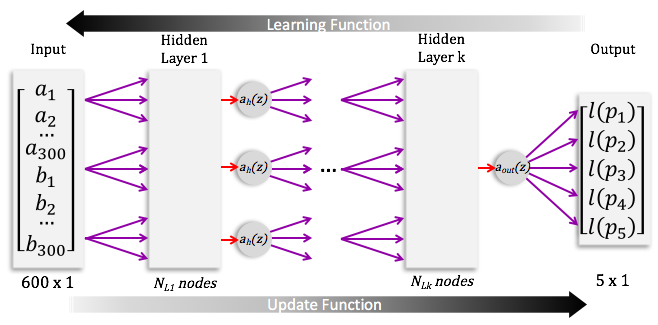
\includegraphics[width=0.7\textwidth]{report_mlp/GenArchitecture.png}}
  \caption{\small A general look at the Neural Network architecture used for a MLP model with $k$ hidden layers with $N_{L_i}$ nodes for the $i$th layer, a common activation function $a_h(z)$ for each layer, and a final output activation function $a_{out}(z)$. The way that these activations propagate through the network is defined by the update function (e.g. simultaneously or sequentially), and the error propagates back according to the learning function. We have 600 features from our input, 1 for each dimension of both entity embeddings, and we are predicting the true/false value of our 5 output predicates. Note that $l(p_1)$ is the likelihood that the predicate $p_1$ is true.  }
  \label{MLPArch}
\end{figure}


\paragraph{}
Much consideration was made in regards to the architecture of the MLP model. These include decisions on how the weights will propagate through the model, how error is propagated back from predictions, and how the first initialization of the weights is determined. A list of these parameters is given below
\begin{center}
\begin{tabular}{|ll|}
\hline
\textbf{Function  }& \textbf{Description } \\%& Examples & Our Choice\\
\hline
\textbf{Activation} & The function applied after each hidden layer. \\%& $\tanh$, Logistic, RELU & Logistic/Sigmoid \\
\textbf{Initialization} & How parameters of the Neural Network are initialized before training. \\%& Random, All 0 or 1, All Positive & Random\\
\textbf{Learning} & How error is propagated from predicted outputs. \\%& Std Back Propagation, BackProp with Momentum &  BackProp with Momentum\\
\textbf{Update} & How the activation functions are propagated through the network. \\%& Simultaneously, In-Order & In-Order (Topologically)\\
\hline
\end{tabular}
\end{center}

We tested different combinations of functions to best suit knowledge graph completion, and ultimately decided on using a sigmoid activation function, random initializations,  backpropagation with momentum to speed up convergence, and a toplogical (in order) method for forward propagation. The sigmoid activation function was chosen for each hidden layer of our MLP architecture because it demonstrated the highest, and most reliable, accuracy than other options such as $\tanh$ or ReLU.

\paragraph{} More importantly, we tested many different architecture sizes. The size includes how many hidden layers, and the size of these hidden layers. To determine this, 
many architectures were tested and the error per iteration for both training and testing sets along with test set ROC curves, were considered in the final determination. These tests are illustrated in the Results section of this report.

\subsubsection{Neural Tensor Network (NTN)}
\paragraph{}  We implemented the Neural Tensor Network (NTN) using TensorFlow 1.3. The architecture was based on \cite{socher2013reasoning}. The scoring function is as follows:

\begin{equation}
g(e_1,R,e_2)  = u_R^Tf \bigg( e_1^TW_R^{[1:k]}e_2 + V_R 
\bigg[ \begin{matrix}  e_1 \\ e_2  \end{matrix} \bigg] + b_R \bigg)
\end{equation}

\paragraph{}  Where  $ W_R^{[1:k]} \in \R^ {d * d * k} $, $ V_R \in \R^ {k * 2d} $, $ b_R \in \R^ {k } $, and  $ u \in \R^ {k } $. d is the size of the embedding and k is the number of slices in the tensor. Each relation $R$ has its own network with the above aforementioned parameters. The model leverages this tensor parameter, $ W_R^{[1:k]} $ to relate the two entity inputs in a multiplicative manner. This is in contrast to the more standard neural network (an MLP leveraging just parameters $ V,u,b $) where the entities are simply concatenated to one another. See Figure \ref{ntn_arch.png} for a visualization. Additionally, all networks share a parameter matrix, $E \in \R^{w*d} $, where w is the number of unique words contained in the knowledge graph, and d representing the embedding size. This parameter is used to determine the entity embeddings as discussed in section 2.2.

\paragraph{}  To train the model, the contrastive max margin loss was minimized:


\begin{equation}
J(\Omega)  = \sum_{i=1}^{N} \sum_{c=1}^{C} max \bigg(0,1 - g\bigg( T^(i) \bigg) +  g\bigg( T_c^(i) \bigg)   \bigg)
\end{equation}

\paragraph{}  Where $ \Omega $ represents the training parameters, $N$ is the number of training samples, $C$ is the corruption size, and $T$ represents the inputs of the triplet to the scoring function. At every training step, each positive triplet, $T$, is duplicated $C$ times. The score for that triplet and then also a corrupted triplet is determined using the neural tensor network scoring function. The corrupted triplet is created by removing either the head entity or tail entity from the triplet with a randomly chosen entity in the entity set. The objective is to increase the margin between the correct and corrupted triplet. We used AdaGrad optimization to train the model. \cite{socher2013reasoning} used L-BFGS optimization; however, this type of optimization does not come with the standard distribution of TensorFlow 1.3.

 \begin{figure}[h!]
\centerline { 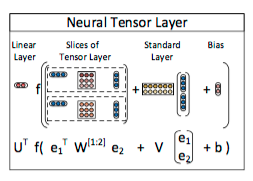
\includegraphics[width=.6\textwidth]{report_ntn/ntn_arch.png}}
  \caption{\small The architecture of the Neural Tensor Network. A layer of the tensor is indicated by a dashed rectangle}
  \label{ntn_arch.png}
\end{figure}

\subsection{Data Curation}


\paragraph{} The dataset we considered was queried from the WikiData, a free opensource knowledge base that acts as the central storage device for its sister projects including Wikipedia, Wikivoyage, and Wikisource \cite{Wikidata}. Wikidata offers a SPARQL type queries for obtaining data on a variety of sources. We queried data regarding the lineage of many famous people in history including: Frederik, Crown Prince of Denmark, George Windsor, Earl of St Andrews, and Shigeko Higashikuni. The relations we considered were if one person, or entity, was the Father, Mother, Spouse, Sibling, or Child of another. See Figure \ref{query} for an example of the query we used to obtain our dataset. 


\begin{figure}[h!]
 \lstinputlisting[language=Matlab]{code/SparqlQuery.txt}
 \caption{\small SPARQL query used to obtain our raw data from Wikidata}
 \label{query}
\end{figure}


\paragraph{} The raw data is a table of values that lists each person and their Father, Mother, spouse, sibling, and child; leaving an entry empty if unknown. We processed this table into positive triplets of the form \texttt{(Q193752, P25, Q229279, 1)} where \texttt{Q193752} and \texttt{Q229279} are a unique encoding of the target and related entities respectively, \texttt{P25} represents one of the relations, or predicates, and \texttt{1} indicates that this statement is true. In english this triplet implies that \texttt{Q229279} is the \texttt{P25} of \texttt{Q193752}. These positive facts represent all the data we can pull directly from the knowledge graphs. However, to increase the robustness of our data, we can create negative facts as well. For example, since we know that Cleopatra VII Philopator, the last active pharaoh of Ptolemaic Egypt, was the daughter of Ptolemy XII Auletes, we can conclude she was not the daughter of Richard Nixon. Thus we can extend our data to contain these negative triplets of the form \texttt{(Q1,P1,Q2,-1)}. In all, we were able to produce 37395 positive triplets and 37391 negative triplets from our raw data. 

\paragraph{} In an effort to exploit the uniqueness in the names for each of our entities, we used word embeddings of each of the words in a name to generate entity embeddings. We used the Fasttext model to generate word embeddings from semantic anaylsis across Wikipedia. Fasttext is a library that represents words as bags of character $n$-grams for fast and efficient classification \cite{BojanowskiGJM16,JoulinGBM16}. Thus, we used Fasttext to obtain $300\times 1$ word embeddings of each of the unique words found in all of our entities' names. For example, the name "Charles Stuart, 1st Earl of Lennox", we found an 300 dimensional embedding vector for Charles, Stuart, 1st, Earl, of, Lennox. Once each of the words had embeddings, we could construct entity embeddings for each of our entities. The method we used for this was to aggregate the word embeddings by taking the mean across each of the words within an entity name. For the MLP model, if Fasttext could not produce a valid embedding for a given word, then that word was ignored. Moreover, if an entity consisted entirely of unknown words, then that entity was thrown out. We did this to preserve the integrity of our input data because in the standard MLP model we would not be training these embeddings. However, for more complex models, another suitable technique is to randomize the embeddings for these entities, or all entities, to guarantee a more representative dataset. Overall, only about 6.4\% of the entities had no suitable embedding. 

\subsubsection{Data staging (MLP)}
\paragraph{}  Once we encoded each entity with their embedding we produced a dataset where each row contains the numeric representation of a triplet. Hence, for a triplet given by \texttt{(EntityA,Pred2,EntityB,1)}, where the embedding for \texttt{EntityA} and \texttt{EntityB }is $[a_1,a_2,\cdots,a_{300}]^T$ and $[b_1,b_2,\cdots,b_{300}]^T$ respectively, the associated row in our data set is given by
$$ \Mat{a_1,a_2,a_3,\cdots,a_{300},b_1,b_2,\cdots,b_{300},0,1,0,0,0} $$
where the last 5 columns represents the truth values for each of the 5 predicates (Father, Mother, Spouse, Sibling, Child).

\subsubsection{Data staging (NTN)}
\paragraph{}  One of the learned parameters for the NTN is the word embeddings. Therefore, before every training step, the entity embeddings had to be recalculated. The word embeddings were represented as a n x d matrix, where n represents the number of unique words across all the entities, and d representing the size of the embedding. Each row index mapped to a unique word. The entity embeddings were then determined by taking the average of the word embeddings that were contained in that entity. The resulting entity embeddings were stored in an n x d matrix, where n was the number of entities across the knowledge graph, and d was the size of the embeddings.

\paragraph{} The training, development, and testing sets contained the triplets, representing a fact in the knowledge graph. The data sets were loaded into an n size matrix, where n was the number of triplets, and each row of the matrix contained the index mapping to the corresponding entity, predicate, as well as the truth value for that triplet. From there, the matrix was grouped into subset matrices corresponding to each predicate.

\subsubsection{Negative Triplets} 
\paragraph{} In an effort to produce harder test cases for our classifiers, for every positive triplet, we created our negative triplet by removing the tail  entity and replacing it with a randomly chosen entity. This limited the negative samples to more realistic test cases. For instance, say there exist a positive triplet, (\textit{Barack Obama, Father, Maliah Obama}). Since Barack Obama has been represented as a Father in this knowledge graph, testing our classifiers on a positive triplet (\textit{Barack Obama, Father, Maliah Obama}) and a negative triplet (\textit{Barack Obama, Father, Chelsea Clinton}) is more realistic than testing the classifier on the test case, (\textit{Maliah Obama, Father, Chelsea Clinton}), given that Maliah Obama has never been represented as a Father in this knowledge graph.  We made sure that this newly constructed triplet did not match a triplet in the positive triplet set. Additionally, we also ensured that the resulting triplet did not have the head entity match the tail entity since that would not make sense for our particular knowledge graph. The resulting number of negative triplets equaled the same number of positive triplets.



\begin{figure}[h!]
\centerline{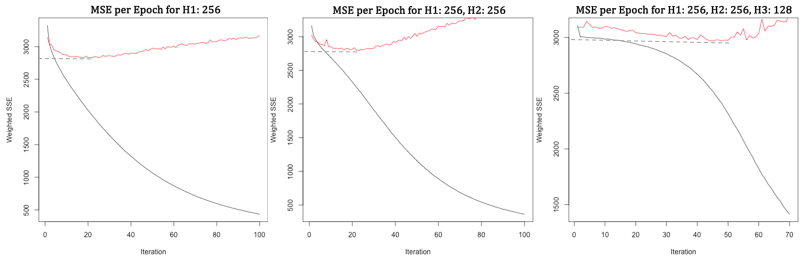
\includegraphics[width=1\textwidth]{report_mlp/MSEperEpochMLP.png}}
  \caption{\small  The weighted SSE after each iteration of the MLP model for 3 different hidden layer architectures. Here both training error (black) and testing error (red) are plotted per epoch, and the min of the testing error is displayed with the dotted line. We noticed that increasing the number of layers only delayed overfitting, but significantly increased its effects once overfitting occured.  }
\label{MSEperEpochMLP}
\end{figure}

\section{Results}
\subsection{MLP}

\paragraph{} We tuned the MLP model significantly in order to handle the complexity of knowledge graph completion. This included determining the best hidden layer architecture and activation functions as well as tuning the learning rate and momentum hyper-parameters.  We test increasing the number of hidden layers as well as the number of nodes per layer.  One statistic we employed for these tests was measuring the weighted SSE after each iteration, where weighted SSE is given as 
$$ SSE = \sum_{k=1}^m \sum_{p=1}^P (p_k - h_\theta(x_k))^2 $$
where we have $m$ sets of triplets, $P$ predicates, and $h_\theta(x_k)$ is the predicted output of the entity-entity pair defined by their concatenated entity embeddings $x_k\in \R^{2 W}$ for $W$ dimensional word embedding sizes. For our MLP model, $m$ is 64950 during the final cross-validation, $W$ is 300, and we have 5 predicates ($P=5$). 

 
\paragraph{} Figure \ref{MSEperEpochMLP} illustrates the change is MSE for each iteration. This shows that for the model with three hidden layers the training error is not decreasing considerably before the 40th iteration. Suddenly, the SSE in this NN structure drops abruptly. The training error, shows that the error keep increasing at that range of iterations. This beahvior, can be attributed to an overfitting in our model.  This trend described above is similar for two hidden layers. For the case of just one hidden layer with 256 nodes, the error does not drop abruptly for the training set but we can see an increase in the error for after 30 iterations, approximately. Moreover, the minimal SSE is smallest with the single hidden layer architecture. These results suggest that only one hidden layer is ideal for our MLP model. Thus, since there is not an improvement in the reduction of error with more layers, and with the benefit of less computational resources being required, we selected single layer architectures moving forward. Note, we tried other sizes for this single layer and found 256 to return the highest specificity, sensitivity, and accuracy when compared with other architectures. 

\paragraph{} Another aspect that is demonstrated in Figure \ref{MSEperEpochMLP} is the overfitting that occurs when the testing error begins to increase. We can notice that under 100 iterations, the training error drops to a weigthed SSE of almost 500. However, our testing error starts increasing after only approximately 30 iterations. From this results, we can infer that we have reached an overfitting in our model and a smaller number of iterations is sufficient. In that sense, future runs consist of around 50 iterations, avoiding the increase in the SSE.

\paragraph{} After deciding which architecture we were to use, we needed to determine the appropriate learning rates and momentum terms for our model. Recall that the update rule for the weights of a Neural Network using backpropagation with momentum is given as 
$$ \Delta w_{ij} (\theta_{i+1}) = -\alpha \delta_{ij}  + \beta \Delta w_{ij} (\theta_i)$$


  \begin{figure}[h!]
\centerline{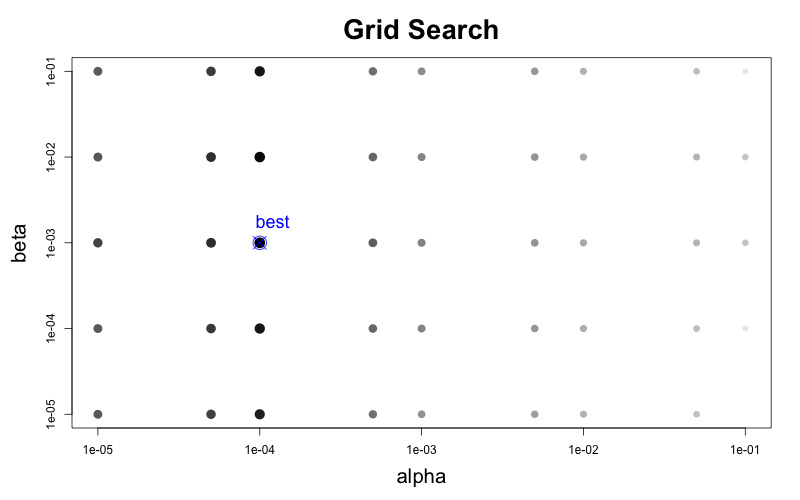
\includegraphics[width=0.6\textwidth]{report_mlp/GridSearch.png}}
  \caption{\small A grid search of the $\alpha$ and $\beta$ hyper-parameters associated with the MLP backpropagation algorithm. Each point represents a full run on the full dataset using an architecture with a single 256 node hidden layer, and the associated mean accuracy is reflected in the transparency of the points. We found the highest accuracy when $\alpha = 1e-4$ and $\beta =1e-3$. }
\label{GridSearch}
\end{figure}

Since the MLP was relatively simple, we determined the best parameters for $\alpha$ and $\beta$ using a grid search method. Figure \ref{GridSearch} shows that the mean accuracy after running a single 256 layer network with each of the associated $\alpha$ and $\beta$ coordinates; where the opacity of the points in the plot is the mean accuracy. This plot shows that a learning rate, $\alpha$, of $1e-4$ and a momentum, $\beta$, of $1e-3$ produced the highest accuracy across the whole dataset. Thus, we used these hyper-parameter values for our full model. 



 
 \paragraph{} Once the full models were determined, we ran a 5-bin cross-validation to truly test our model. Figure \ref{ROC-Curve} shows the ROC curves for using both randomly initialized embeddings and Fasttext pre-trained embeddings as the inputs to the model. Notice that the sensitivity, or true positive rate, suffers from the random embeddings. The model with random embeddings heavily biases false negative calls in order to guarantee the vastly disproportional true negative calls for the MLP dataset. A problem decreased by the pre-trained embeddings. Moreover, the accuracy for this is shown in Table \ref{accuracy}.  
 

 
\subsection{NTN}
\paragraph{} Given the computationally intensive task of training the NTN (could take over 8 hours to see convergence in the loss), a less rigorous hyperparameter optimization was performed. Starting with similar hyperparameter values that  \cite{socher2013reasoning} used, we implemented a variety of NTN models with differing hyperparameters and found that setting the corruption size to 10, tensor layer slice size to 3, L2 regularization set to .0001, and a 0.01 learning rate provided respectable results. For each implementation, we cross validated over a development set to determine the classification threshold for each relation network. See figure \ref{_loss_.pdf} of the loss with respect to training step iterations. We found that around 1000 training steps with a batch size of 10000 samples provided sufficient training for both the randomly and pretrained initialized word embeddings.

 \begin{figure}[h!]
\centerline{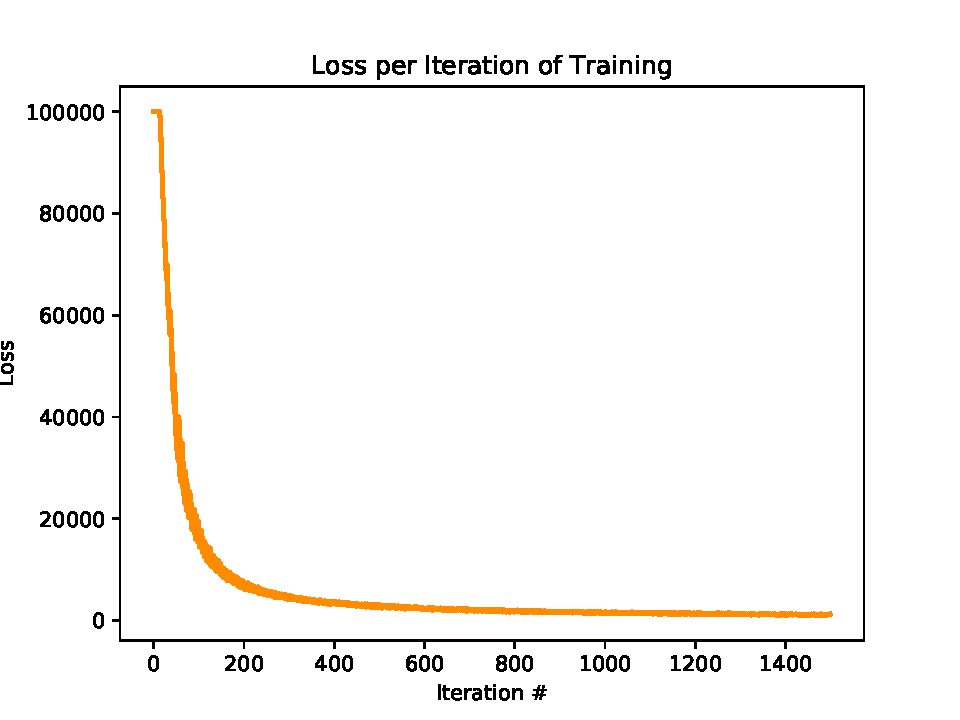
\includegraphics[width=0.5\textwidth]{report_ntn/_loss_.pdf}}
  \caption{\small Plots of the contrastive max margin loss with respect to iteration of training. The loss converged at around 1000 training steps. }
\label{_loss_.pdf}
\end{figure}

\paragraph{} Also of interest, is the noticeable clustering of the word embeddings after training the model. See the appendix for Figure \ref{tSNE} of the model with randomly initialized word embeddings. Both tSNE plots show the same 500 word embeddings before and after training. The colors of the words indicate the k means cluster that the words end up resulting in on the final iteration. These clusters of the word embeddings that are occurring indicate a learned semantic relationship with one another.

\paragraph{}  See Figure \ref{ROC-Curve} for the ROC curve for the NTN model. The ROC curve for the randomly intialized word embeddings showed a respectable 0.906 AUC. Additionally, as can be seen in table \ref{accuracy}, with the exception of the spouse classification, all accuracies were 80\% or higher, with the overall accuracy being 88\%. With respect to the MLP implementation, these are very respectable results. 

\paragraph{}  However, One will quickly notice that the pretrained word embedding model actually performed worse than the randomly initialized word embedding model. This more than likely occurred due to the large portion of words contained in the entities were missing from the pretrained FastText embedding model. We only saw a total of 1735 words from the FastText pretrained model that matched the over 6035 unique words found in the entities. Due to this, we had to drop 2305 entities since there was no word contained in the respective entity that was found in the pretrained model. Additionally, given that we dropped a word from the entity if we did not have a match in our pretrained model, we had over 50\% of the entities have at least one other duplicated embedding value with respect to another entity. Although this is not an ideal testing condition for the neural tensor network over pretrained word embeddings, we still found it intriguing that the results were actually worse than the randomly initialized word embedding model. This further argues, in line with \cite{socher2013reasoning}, that the initialization technique performed on the word embeddings plays a powerful role in the performance of this model.

 \begin{table}[h!]
\begin{center}
\begin{large}
Accuracy for Each Model
\end{large}
\begin{tabular}{|cc|ccccc||cc|}
\hline
\textbf{Model} & \textbf{Embeddings} & \textbf{Father} & \textbf{Mother} & \textbf{Sibling} & \textbf{Spouse} & \textbf{Child} & \textbf{ Overall} & \textbf{Std-Dev}\\
\hline
NTN & Random 		&	0.891 	& 0.872 	& 0.926	&	0.773	&  0.880	& \textbf{0.881}	 & 0.057	\\
NTN & Pre-Train 		&	0.850 	& 0.821 	&	0.853	& 0.789	& 0.809 	& \textbf{0831}	& 0.027	\\

MLP & Random 		& 0.828 & 0.829 & 0.823 & 0.660 & 0.719 &  \textbf{0.772}	& 0.078	\\
MLP & Pre-Train 		& 0.915 & 0.917 & 0.906 & 0.749 & 0.805 & \textbf{0.858}	& 0.077	\\
\hline
\end{tabular}
\end{center}
  \caption{\small Table illustrating the accuracy for each of the predicates we classified on. Notice the NTN model had the highest accuracy with randomly initialized word embeddings, but with so many missing word embeddings, initializing the model with pre-trained embeddings caused the accuracy to drop. The MLP model proved to be more robust to these bad embeddings and had a significant increase in accuracy with pre-trained embeddings.  Moreover, the variation in the accuracies between the NTN and MLP models is significant as shown by the standard deviation. }
  \label{accuracy}
\end{table}

\begin{figure}[h!]
\centerline{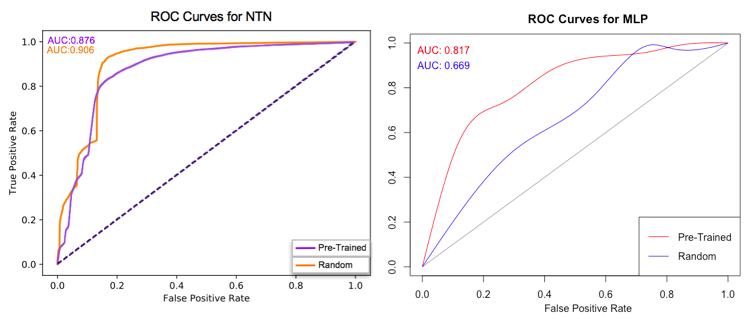
\includegraphics[width=1\textwidth]{report_mlp/ROC-Curves.png}}
  \caption{\small  A comparison of the ROC curves between Random and Pre-trained word embedding initializations  for the entity embedding construction of the NTN and MLP models. The different points were obtained through 5-bin cross-validation for each of the 5 predicates; with the AUC is computed using natural cubic splines. }
\label{ROC-Curve}
\end{figure}

\section{Discussion}

\subsection{Implementation and Training}
\paragraph{} The relative simplicity of an MLP implementation is attractive compared to the complexity of an NTN. In an MLP implementation, adjusting hyperparameters is simple and ease of training allows for quick reevaluations. Furthermore, the training time was significant between the two; the MLP model converges in a few hundred iterations and trained in about 1.5 hours as compared to the NTN which could take over 8 hours to converge. This is expected as an NTN requires tuning the additional weights for the word embeddings and the bilineal tensor layer when compared to the MLP model.

\paragraph{}The cost of NTN training was significantly more than MLP; this permitted exploring more hyperparameters, test more hidden layer architectures, various activation functions, and backpropagation routines. Improving the training costs for NTN would provide potential improvements by finding more optimal hyperparameters and architectural design features. While the training time favors MLP, the results demonstrated that this training time was worthwhile.

\subsection{Precision and Pretrained Embeddings}
\paragraph{} The NTN model, implemented in  TensorFlow, provides a high true positive to false positive rate. While the accuracy is not as high as anticipated, there are several ways we could improve this. Due to consistency issues between the pretrained and data embeddings (duplicates and misspellings), our NTN trained on 2300 less embeddings and had lower accuracy than random embeddings. We can likely improve our loss by improving the consistency of our data and pretrained embeddings. Our pretraining was likely a limiting factor, and the quality of the pretrained model imposed a distinct disadvantage to random initialization. This demonstrates the effectiveness of good pretraining.

\paragraph{} MLP with random initialized word embeddings performed worse than NTN with random initialized word embeddings. However MLP was more robust initially to bad pretrained embeddings and improved by almost 10\% accuracy. 

\paragraph{} While negative triplets prove to be an effective tool there was a lack of consistent symmetry in our data. Providing a completed set of complementary relationships could provide better validation results. However, enforcing strict symmetry throughout a knowledge base is extremely unrealistic and won't provide a significant enough improvement for low relational entities.

\paragraph{} In our analysis of both MLP and NTN we can deduct reasons for choosing each of the models. When training time is of concern and design iterations need to happen more frequently, MLP can be a better solution. However, NTN demonstrated better precision at a cost of training time.

\pagebreak
\bibliographystyle{ieeetr}
\bibliography{bib}{}

\pagebreak
\section*{Appendix}
\begin{figure}[h!]
\centerline{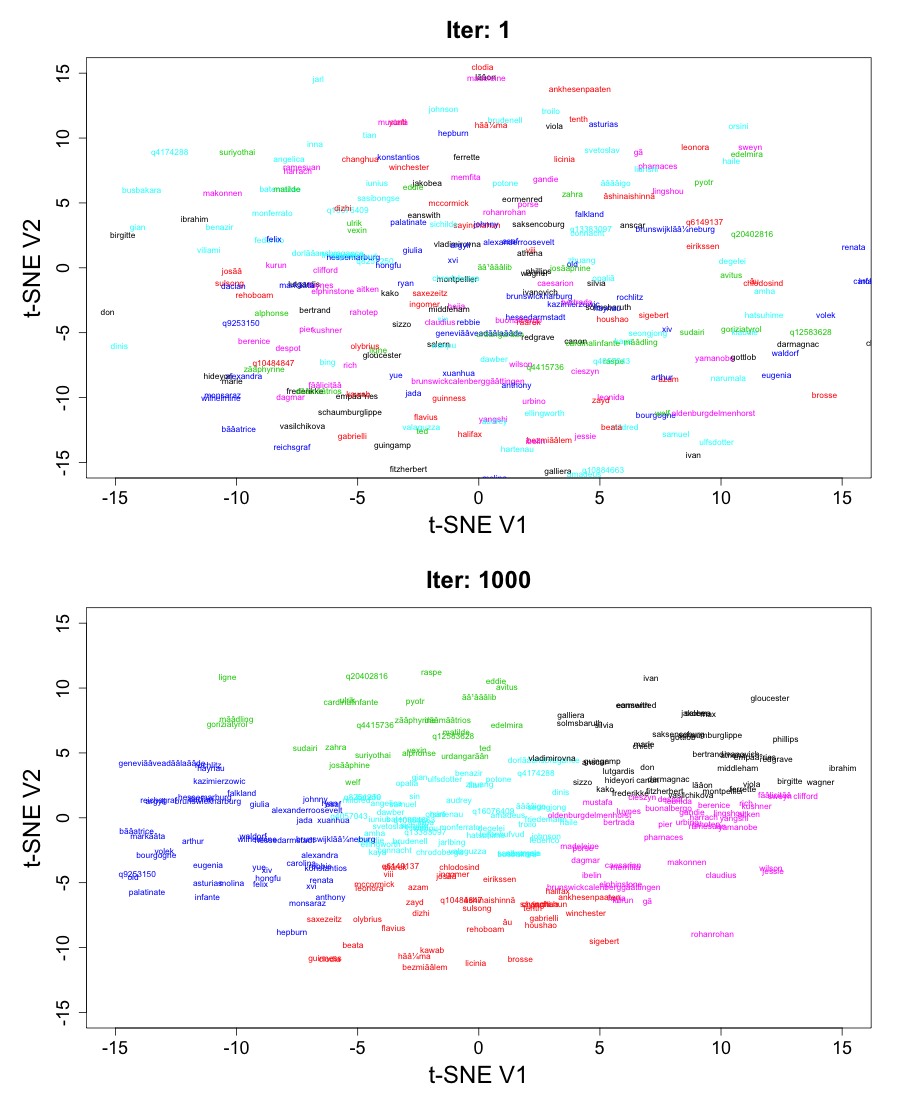
\includegraphics[width=0.95\textwidth]{report_ntn/FirstLast-tSNE.png}}
  \caption{\small  The word embeddings both before and after training the NTN model on randomly initialized embeddings. The clustering is performed using k-Means to show how much each embedding has changed. }
\label{tSNE}
\end{figure}


\end{document}
